\section{Results}
\label{sec:results}

In this section the results of the tests described in section~\ref{sec:evaluation_and_testing} will be discussed. These results should provide knowledge about the correctness of the implementation in relation to the requirements specified in section~\ref{sec:requirements}.

As mentioned, the white box tests were derived from Raft's behaviour in its condensed summary in the paper. The output of these tests is listed in appendix~\ref{sec:results}.
The black box tests, however, were only done for a given set of scenarios in order to show that the fault tolerant features of the implementation reflects those described in the paper.

\subsection{Running the simulator}
On top of the tests, a simulator that visualizes the implementation was done in order to get illustrative feature to show how Raft solves the consensus problem in presence of faulty servers. The screenshot in figure~\ref{fig:example1}belows shows a run of the simulator.

\begin{figure}[H]
\centering
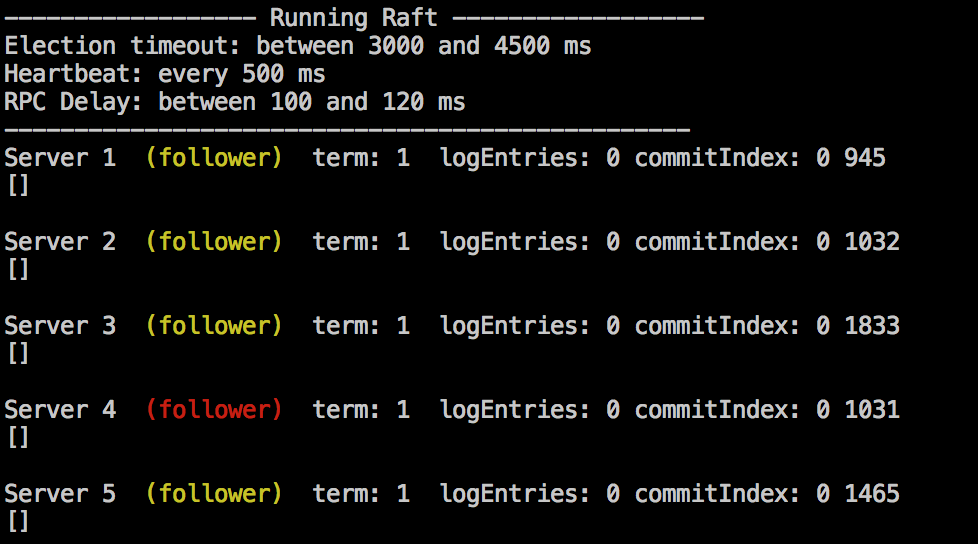
\includegraphics[scale = 0.5]{screenshot-coming-leader-election}
\caption{Example run of the simulator in the state where a leader has not yet been elected.}
\label{fig:example1}
\end{figure}

The simulator lists the servers by their id, state, the amount of entries in its log, its latest commit index, and its time out which decrements. Server 4 is colored red to illustrates that it has crashed.
The screenshot in figure~\ref{fig:example2} then shows the situation where a server times out and starts an election by transitioning to the candidate state and requesting votes from the other servers.

\begin{figure}[H]
\centering
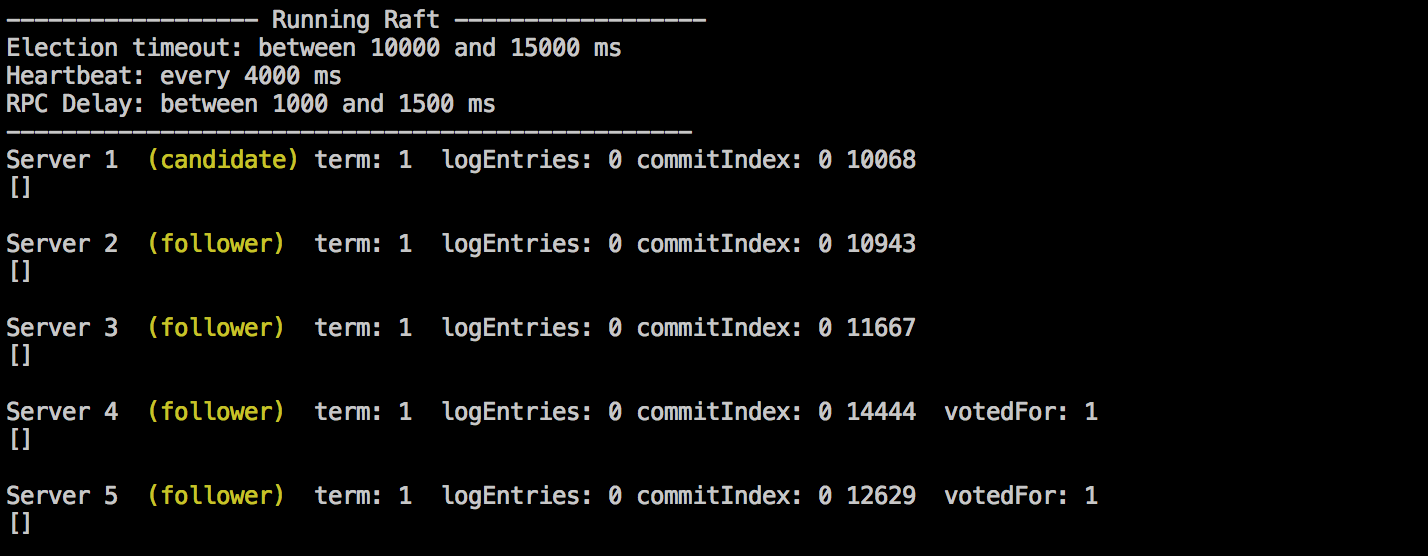
\includegraphics[scale = 0.5]{screenshot-ongoing-leader-election}
\caption{Example run of the simulator in the state where a server has started an election.}
\label{fig:example2}
\end{figure}

And lastly the screenshot in figure~\ref{fig:example3} shows the situation in which a crashed server hasn't had its log updated since the leader does not get replies from the heartbeat messages it send to it.

\begin{figure}[H]
\centering
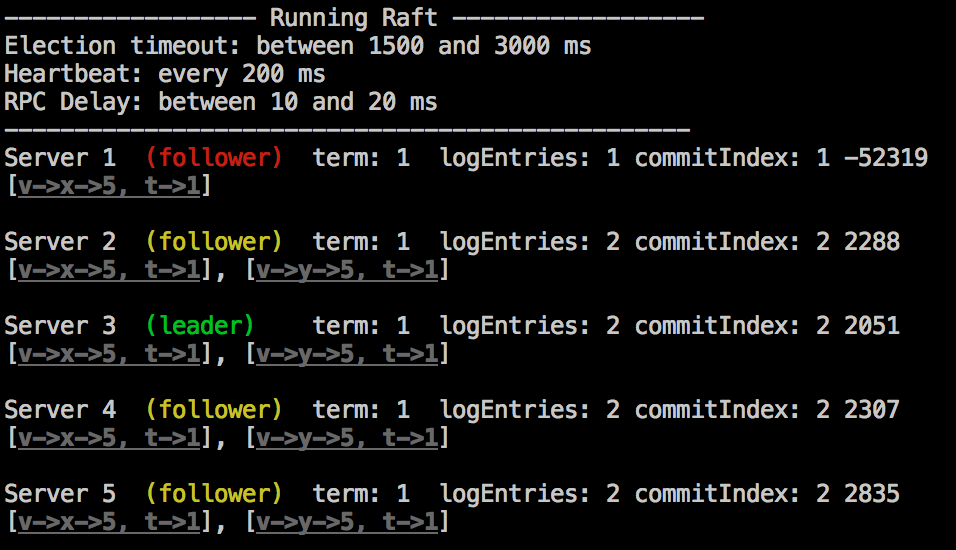
\includegraphics[scale = 0.5]{screenshot-outdated-crashed-server}
\caption{Example run of the simulator where a leader has been elected and request from a the client has been replicated to all correct servers.}
\label{fig:example3}
\end{figure}
These screenshots of a run of the simulator serves as results of the acceptance tests.
Furthermore a video of running the simulator can be seen in the following link:\\ \url{https://www.dropbox.com/s/75kpa65yykld2mv/simulator_run_video.mov?dl=0}.

The output results of the both the white box and black box test are given in appendix~\ref{sec:results_app}.

\subsection{Visualization} % (fold)
\label{sub:visualization}

The raft implementation, raft simulator and command line visualization are seperated in three reuseable compontens. This means that a another GUI visualization such as in a browser would be easy as the raw raft implementation and simulator can be reused together with a browser visualization module.

The command line visualization is implemented using an HTTP-server that runs with the raft visualization process. To manipulate with the visualization the raft client sends an HTTP-request, which the command server receives and invokes the relevant method on the visualization process.

% subsection visualization (end)

\subsection{Source Code} % (fold)
\label{sub:source_code}

Can find it through a ZIP-file and on GitHub.

The source code has been attached as appendix on CampusNet as a ZIP-file, but it can also be accessed through GitHub at the url:

{\setlength\parindent{24pt} \href{http://github.com/anderslime/ft-raft}{http://github.com/anderslime/ft-raft}

% subsection source_code (end)
